\subsubsection{How the OpenDwarfs N Body Implementation works}
\par{Host code, {\color{red}shown in listing \ref{nbody_host}}, calls kernel code multiple 
    times based on the number of global work items declared and 
    the number of vertices on the surface of the selected bio molecule. There are 30 arguments passed 
    to the kernel, with 16 of these being \_\_global CL\_MEM\_READ\_ONLY buffers and 1 being \_\_global CL\_MEM\_READ\_WRITE 
    buffer for the final output.}

\par{Every work item in OpenCL is an implementation of the kernel code. 
    Hence each work item does a single step n body calculation. i.e. 
    Each work item is working on the total electrostatic potential on a vertex due to the atoms.}

\par{The kernel code, {\color{red}shown in listing \ref{nbody_kernel}}, 
    executes a regular computation pattern, with each work item per work group 
    performing the same computation. This results in no dependencies that may hinder computation continuity. 
    Computations include divsion and square root operations on floating point numbers which is an expensive bottleneck. 
    {\color{red}A graphical representation of this is shown in figure \ref{nbody_graph}.}}

\begin{figure}[!h]
    \centering
    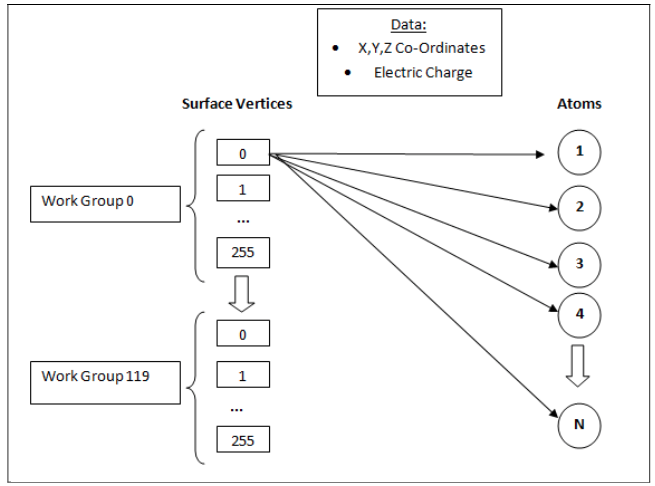
\includegraphics[width=0.5\textwidth]{figures/graph_nbody.png}
    \caption{Graphical representation of kernel code.}
    \label{nbody_graph}
\end{figure}

\par{\textbf{Within the Kernel}}
\par{The distance r is key here, as it decides (using conditionals) the type of calculation 
    to be done on the point of interest. The value of r is compared against rprime (Threshold 
    for the ion exclusion radius) and A. If r > rprime, then the atoms are considered as distant 
    components. If r<A, then 0 < dist\_to\_surf <= ion\_excl\_rad. Otherwise the point is considered 
    to be on the surface (a vertex) of the molecule. With the tests that have been run on this code, 
    the preset value for p was 0.0. This resulted in only one set of conditionals ever being executed 
    in the code. This is a possible case for inefficiency as discussed later.}

\par{Based on the processor in use, making changes to the work group sizes can greatly affect the
    efficiency and speed of the program. As with any kernel, optimising the code to fit the hardware 
    is essential. Understanding the hardware is an essential part of OpenCL code development.}

\subsubsection{H2D and D2H times}
\par{Host to Device and Device to Host time changes based on the size of the file to be processed. 
    With a larger file comes a larger transfer time. This is as expected. 
    There are small variations in the H2D and D2H time based on changes with 
    Global and Local Work Item sizes in 0 and 1 dim but these do not seem to change considerably.}

\subsubsection{Bio Molecules tested}
\begin{itemize}
    \item \textbf{NUCLEOSOME}: This molecule contains 1268 residues\footnote{is recognizable molecular 
                            part of a larger molecule(an atom or group of atoms considered as a group 
                            or part of a molecule.). This is the structural component within a molecule 
                            which is exploited} and 25086 atoms. Total molecular charge of -144.00.
                            Molecular surface consists of 258797 vertices and 517826 triangles,
                            the estimated electrostatic radius (A) of this molecule is: 51.1889.
    \item  \textbf{CAPSID}: This molecule contains 30780 residues and 476040 atoms. Total molecular charge of 236.35
                            Molecular surface consists of 593615 vertices and 1187226 triangles,
                            the estimated electrostatic radius (A) of this molecule is of 164.262.
\end{itemize}



